\documentclass[a4paper]{scrartcl}
\usepackage[cm]{fullpage}
\usepackage{amsmath, amssymb, esint}
\usepackage{siunitx}

\usepackage{tikz, pgfplots, pgfplotstable}
\pgfplotsset{
    compat = 1.12,
    plot-scatter/.style = {
        only marks,
        error bars/.cd,
        x dir = both, y dir = both,
        x explicit, y explicit
    }
}

\pgfplotstableread{data/results.tsv}\resultstsv

\begin{document}

\title{PHYS3112: Zeeman Effect}
\author{ \\ \\ }
\date{2017-05-17}
\maketitle

\begin{abstract}
    The Zeeman effect is observed for a Cd I's \SI{643.8}{\nano\metre} line, to both observe the polarisation of light due to the effect, and to calculate a value for the Bohr magnetron. Of the triplet produced by the Zeeman effect, the center line is linearly polarised parallel to the applied magnetic field, while the other two lines are orthogonally circularly polarised in the plane orthogonal to the field. Meanwhile, our value for the Bohr magnetron is 1.6 the expected value, indicating possible specification errors.
\end{abstract}

\section{Materials and Methods}
Please refer to the student notes and operating instructions of the experiment.

A Moticam 1 was substituted for the camera mentioned in the operating instructions. It has a resolution of \(800 \times 600\) pixels with an imaging area of \(3.58 \times 2.69 \si{\milli\metre}\), corresponding to \SI{4.49}{\micro\metre} per pixel. In practice, this value doesn't matter, since we will be using a method that is independent of image scale.

The radii of interference rings was found by the following steps on the captured image:
\begin{enumerate}
    \item Taking an adaptive threshold (with \emph{Mathematica 10.2}'s \texttt{LocalAdaptiveBinarize[image, 5]})
    \item Find the connected components (\texttt{MorphologicalComponents[image]})
    \item Using the components that correspond to each ring to mask the original image
    \item Performing a least squares fit of a circle, weighted by the greyscale channel value (note: not gamma corrected, so not as effective as it could be)
    \item Calculating the circle radius and standard error from the fit
\end{enumerate}

The output of the etalon and imaging lens will have interference maxima following the criteria:
\[(k_0 + k) \lambda = 2 d \cos \theta = 2 d \cos \tan^{-1} \frac{r}{f} = \frac{2 d}{\sqrt{1 + \frac{r^2}{f^2}}}\]
where \(k_0\) is an arbitrary integer, \(k\) is the interference order, \(d\) is the air gap of the etalon, \(r\) is the circle radius, and \(f\) is the focal length of the imaging lens.

Let us define \(\varepsilon = \lim_{r \to 0} k\), called the fractional order:
\[\varepsilon = \frac{2 d}{\lambda} - k_0\]

If we take the difference of the fractional orders of the larger and smaller interference circles, we can find the energy shift between them:
\begin{align*}
    \Delta \varepsilon &= 2 d \Delta\left(\frac{1}{\lambda}\right) \\
    &= 2 d \Delta\left(\frac{E}{h c}\right) \\
    &= \frac{2 d}{h c} \Delta E_{\Delta \varepsilon}
\end{align*}

Remembering that the energy difference between the larger and smaller interference circles are double the energy difference between individual lines of the Zeeman effect, we obtain:
\[\Delta E_{\Delta m = \pm 1} = \frac{\Delta E_{\Delta \varepsilon}}{2} = \frac{h c}{4 d} \Delta \varepsilon\]

Using our results from the prework, we can solve for the Bohr magnetron via a linear regression:
\[\left(\mu_B \frac{4 d}{h c}\right) B = \left|\Delta \varepsilon\right|\]

How can we actually find \(\varepsilon\)? The student notes says to take the linear regression of:
\[m r^2 + \varepsilon = k\]
where the resulting \(m\) is discarded, since we only want \(\varepsilon\).

\section{Results}
\begin{figure}
    \centering
    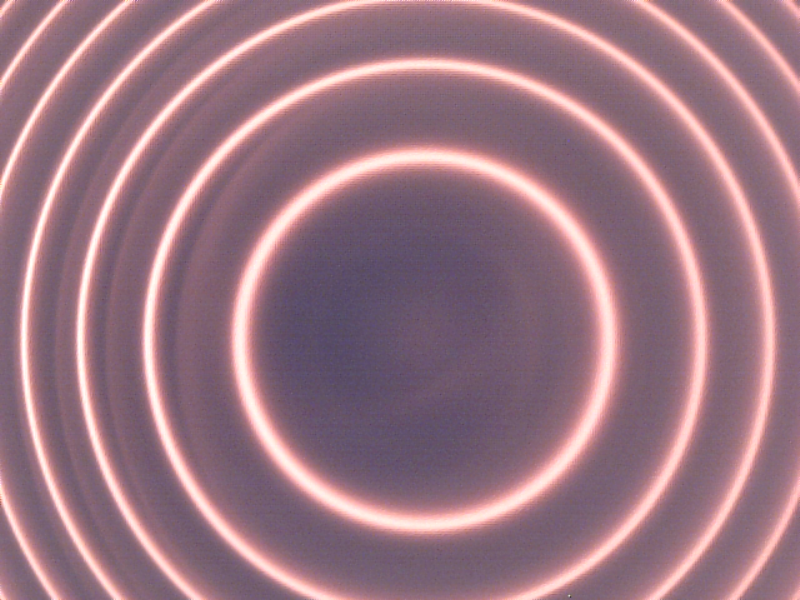
\includegraphics[height = 10cm]{data/0mT-orth.png}
    \caption{Captured rings orthogonal to the field at \(B = \SI{0}{\milli\tesla}\)}
    \label{fig:zero-rings}
\end{figure}
\begin{figure}
    \centering
    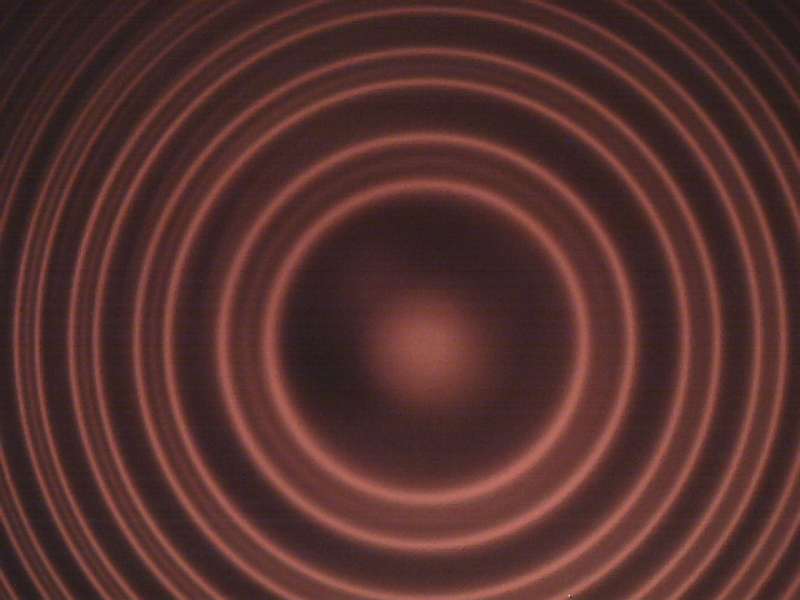
\includegraphics[width = 8cm]{data/475+-10mT-parr.png}
    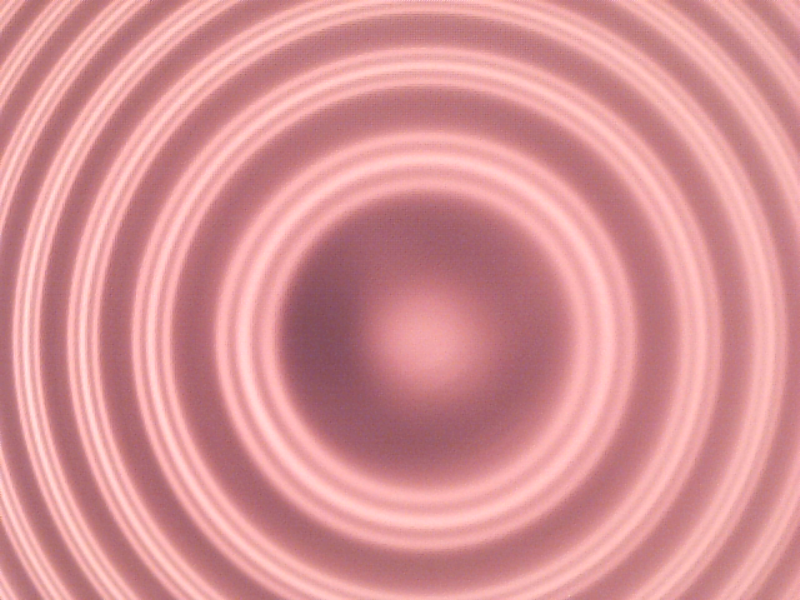
\includegraphics[width = 8cm]{data/475+-10mT-orth.png}
    \caption{Captured rings parallel and orthogonal (respectively) to the field at \(B = \SI{475 \pm 10}{\milli\tesla}\)}
    \label{fig:zeeman-rings}
\end{figure}
\begin{figure}
    \centering
    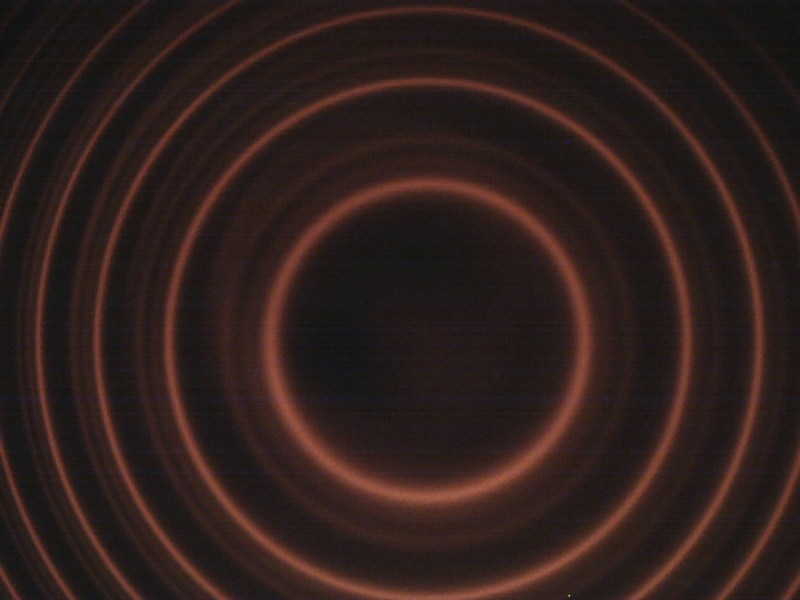
\includegraphics[width = 8cm]{data/475+-10mT-parr-north-away-circular-polariser.png}
    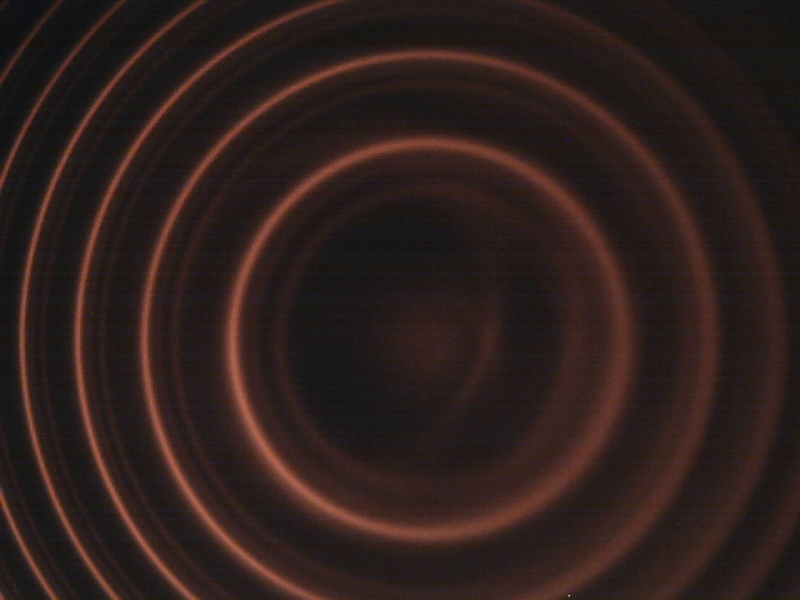
\includegraphics[width = 8cm]{data/475+-10mT-parr-north-towards-circular-polariser.png}
    \caption{Captured rings parallel to the field at \(B = \SI{475 \pm 10}{\milli\tesla}\) with orthogonal circular polariser configuartions}
    \label{fig:circular-polariser}
\end{figure}
\begin{figure}
    \centering
    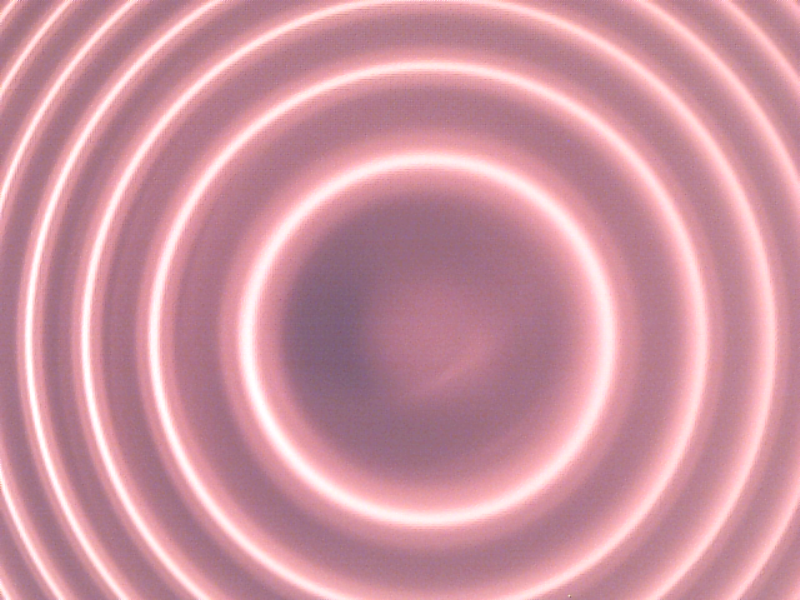
\includegraphics[width = 8cm]{data/475+-10mT-orth-linear-polariser-parallel.png}
    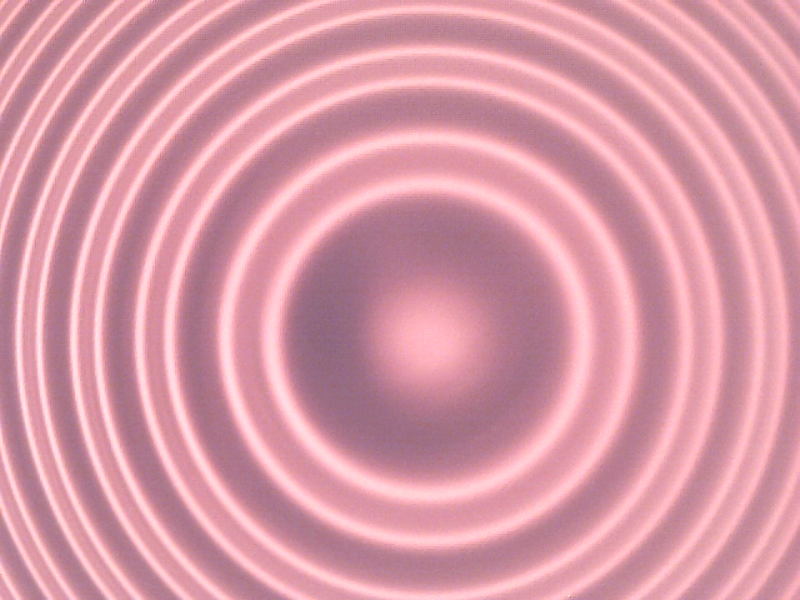
\includegraphics[width = 8cm]{data/475+-10mT-orth-linear-polariser-orth.png}
    \caption{Captured rings orthogonal to the field at \(B = \SI{475 \pm 10}{\milli\tesla}\) with linear polariser parallel and orthogonal to the field, respectively}
    \label{fig:linear-polariser}
\end{figure}

\begin{figure}
    \centering
    \begin{tikzpicture}
        \begin{axis}[
            xlabel = \(B\) (\si{\milli\tesla}),
            ylabel = \(\Delta \varepsilon\)
        ]
            \addplot +[plot-scatter] table [
                x expr = \thisrowno{0},
                x error expr = \thisrowno{1},
                y expr = \thisrowno{2},
                y error expr = \thisrowno{3}
            ] {\resultstsv};
            \addplot +[no marks, domain = 175:500] {-0.0161762 + 0.000875683 * x};
            \addplot [no marks, domain = 175:500] {-0.0221253 + 0.000860028 * x};
            \addplot [no marks, domain = 175:500] {-0.010227 + 0.000891337 * x};
        \end{axis}
    \end{tikzpicture}
    \caption{Measured \(B\) against calculated \(\Delta \varepsilon\), along with its linear regression}
    \label{fig:results}
\end{figure}

When a magnetic field was applied to the source, the interference rings of no field (Figure \ref{fig:zero-rings}) split into a doublet when observed parallel to the field, into a triplet when observed orthogonal (Figure \ref{fig:zeeman-rings}). A larger field strength caused a greater splitting.

When a circular polariser was applied when viewing the source in parallel with the field, the inner and outer rings (of each order) can be observed to have orthogonal circular polarisations (Figure \ref{fig:circular-polariser}).

When a linear polariser was applied when viewing the source orthogonal to the field, the central ring was observed to be polarised parallel to the field, while the other two rings were polarised orthogonal to the field (Figure \ref{fig:linear-polariser}).

Note that even though certain orientations of the field and polarisers decreased the intensity of certain lines significantly, they can still be faintly seen.

For each magnetic field strength used, four interference orders were captured parallel to the field and measured without the polariser. Each order's rings consisted of a pair of rings, as can be seen in Figure \ref{fig:zeeman-rings}.

The fractional order \(\varepsilon\) was calculated individually for both the larger and smaller of the pair, and subtracted to produce \(\Delta \varepsilon\) for each field setting. These fractional order differences are then plotted against the field setting, and a linear regression taken, as can be seen in Figure \ref{fig:results}.

The fitted line had a gradient of \SI{8.76 \pm 0.16e-4}{\per\milli\tesla}, corresponding to a Bohr magnetron of \SI{90.5 \pm 1.6}{\micro\electronvolt\per\tesla}. This is approximately 1.6 times the accepted value for the Bohr magnetron of \SI{57.9}{\micro\electronvolt\per\tesla}.

\section{Discussion}
The Zeeman effect exists, as can be seen from the line splitting when a magnetic field is applied.

From the polarisation observations in Figures \ref{fig:circular-polariser} and \ref{fig:linear-polariser}, one can conclude:
\begin{itemize}
    \item The central ring is linearly polarised parallel to the applied field, and hence cannot be observed when viewing the source in parallel to the field, since no longitudinal polarisation for light exists.
    \item The other two rings are orthogonally circularly polarised, with the ``plane of rotation'' being orthogonal to the field axis, and hence can be seen from all observation axes. 
\end{itemize}

The ``leakage'' of the lines, despite being significantly attenuated due to the orientation of the field or polarisers, are most likely due to reflections or higher order electron transitions (i.e., not electronic dipole), and hence are not completely attenuated.

While our value for the Bohr magnetron is 1.6 times the accepted value, it is within the correct order of magnitude so our quantitative results are not completely absurd. In fact, using a completely different method to calculate the Bohr magnetron from the same data produced the same value, indicating our analysis method is fine. More likely, some given equipment parameters are probably incorrect, such as the etalon spacing \(d\), or even the \(g\)-value for the two Cadmium energy levels.

\section{Conclusion}
\emph{(From abstract)} The Zeeman effect is observed for a Cd I's \SI{643.8}{\nano\metre} line, to both observe the polarisation of light due to the effect, and to calculate a value for the Bohr magnetron. Of the triplet produced by the Zeeman effect, the center line is linearly polarised parallel to the applied magnetic field, while the other two lines are orthogonally circularly polarised in the plane orthogonal to the field. Meanwhile, our value for the Bohr magnetron is 1.6 the expected value, indicating possible specification errors.

\end{document}